\documentclass[10pt,letterpaper]{article}
\usepackage[top=1in,bottom=1in,left=1in,right=1in]{geometry}
\usepackage{datetime}
\usepackage{natbib}      % http://merkel.zoneo.net/Latex/natbib.php
\usepackage{palatino}
\usepackage{verbatim}
\usepackage[normalem]{ulem}
\bibpunct{(}{)}{;}{a}{,}{,}

\usepackage{array}

\usepackage{chngpage}
\usepackage{stmaryrd}
\usepackage{amssymb}
\usepackage{amsmath}
\usepackage{graphicx}
\usepackage{lscape}
\usepackage{subfigure}
\usepackage[usenames,dvipsnames]{color}
\definecolor{myblue}{rgb}{0,0.1,0.6}
\definecolor{mygreen}{rgb}{0,0.3,0.1}
\usepackage[colorlinks=true,linkcolor=black,citecolor=mygreen,urlcolor=myblue]{hyperref}

\newcommand{\bocomment}[1]{\textcolor{Bittersweet}{BO says: #1}}

\newcommand{\ignore}[1]{}
\newcommand{\transpose}{^\mathsf{T}}
\newcommand{\inner}[1]{\langle #1 \rangle} 
\newcommand{\smallsec}[1]{\noindent \textbf{#1\ }}
\newcommand{\cmd}[1] {{\color{blue}\texttt{#1}}}

\newcommand{\solution}[1]{{\color{myblue} \emph{[Solution:} 

#1 

\emph{End solution]}}}
\newcommand{\solutionnote}[1]{{\color{myblue} \emph{[Note:}

#1 

\emph{End note]}}}
\newcommand{\points}[1]{{\color{mygreen}\emph{[#1]\ \ }}}

\newcommand{\aone}{\diamondsuit}
\newcommand{\atwo}{\heartsuit}
\newcommand{\bone}{\triangle}
\newcommand{\btwo}{\Box}
\newcommand{\myand}{\ \land\ }
\newcommand{\myor}{\ \lor\ }
\newcommand{\mynot}{\lnot}

\title{
  Homework 5 \\
  \Large{CMPSCI 370 Spring 2018, UMass Amherst} \\
  \Large{Due: April 25, 11:55 PM} \\
  \Large{Instructor: Subhransu Maji} \\
  \Large{TA: Tsung-Yu Lin}
}

\settimeformat{ampmtime}
\date{}
\begin{document}
\maketitle

\renewcommand\thesubsection{\thesection.\alph{subsection}}


\section*{Guidelines}


\paragraph{Submission.} Submit your answers via Gradescope that includes a pdf with your solutions and source code. You have a total of 5 late days for all your homework assignments which you can use in any way you like. However note that delay by even one minute counts as a full late day and submissions beyond the late days will not be given \emph{any} credit. Please contact the instructor and obtain permission ahead of time if you seek exceptions to the policy.

\paragraph{Plagiarism.} We might reuse problem set questions from previous years, covered by papers and webpages, we expect the students not to copy, refer to, or look at the solutions in preparing their answers. We expect students to want to learn and not google for answers. Any instance of cheating will lead to zero credit for the homework, and possibly a failure grade for the entire course.

\paragraph{Collaboration.} The homework must be done individually, except where otherwise noted in the assignments. 'Individually' means each student must hand in their own answers, and each student must write their own code in the programming part of the assignment. It is acceptable, however, for students to collaborate in figuring out answers and helping each other solve the problems. We will be assuming that you will be taking the responsibility to make sure you personally understand the solution to any work arising from such a collaboration.

\paragraph{Matlab requirements.} The code should work any Matlab version ($\geq$ 2011a) and relies on the Image Processing Toolbox for some functions.

\paragraph{Python requirements.} We will be using Python 2.7. The Python starter code requires \cmd{scipy}, \cmd{matplotlib} and \cmd{pillow} for loading images and \cmd{numpy} for matrix operations (at least v1.12). 
If you are not familiar with installing those libraries through some package manager (like \cmd{pip}), the easiest way of using them is installing \href{https://conda.io/docs/user-guide/install/index.html}{Anaconda}. Contact the course staff if you are having trouble installing these.

\paragraph{Using other programming languages.} We made the starter code in Python and Matlab. You are free to use other languages such as Octave or Julia with the caveat that these will not be supported by the course staff.

\newpage

\section*{The MNIST dataset}
In this homework you will train a decision tree classifiers to predict whether an image is a $3$ or a $8$. The dataset for this homework can be loaded into Matlab by typing $\cmd{load(data.mat)}$. In Python, you can use the function $\cmd{loadmat}$ in $\cmd{utils.py}$ to store the data in a variable. E.g., $\cmd{data = utils.loadmat('data.mat')}$. The data is split into $\cmd{train}$ and $\cmd{test}$ sets.

For each split, the features and labels are in variables $\cmd{x}$ and $\cmd{y}$ respectively. E.g., $\cmd{data.train.x}$ is an array of size $28 \times 28 \times 1 \times200$ containing $200$ digits.
In Python, data is organized as a dictionary (i.e. $\cmd{data["train"]["x"]}$) and the array has size $28 \times 28 \times 200$. There are 100 digits each from classes ${3}$ and ${8}$, each of size $28 \times 28$. 
Class labels are given by the variable $\cmd{data.train.y}$. Thus, pixel \cmd{(i,j)} in the the \cmd{k'th} training example is \cmd{data.train.x(i,j,1,k)} with label \cmd{data.train.y(k)}. In Python, the same pixel can be accessed thorugh \cmd{data["train"]["x"][i, j, k]} with label \cmd{data["train"]["y"][k]}. The $\cmd{test}$ set contains $100$ examples from the two class in the same format. This data is a subset of the much larger MNIST dataset~\footnote{\url{http://yann.lecun.com/exdb/mnist/}}.

The features are simply the binary pixel values, i.e., each pixel is either 0 or 1. You can visualize the dataset using $\cmd{montageDigits(x)}$ function. Below is the output of $\cmd{montageDigits(data.train.x)}$. \textit{Tip: $\cmd{montageDigits(x)}$ internally uses the $\cmd{montage}$ command in Matlab which has a $\cmd{size}$ option controlling the number of rows and columns of the output.}

\begin{figure}[h]
\centering
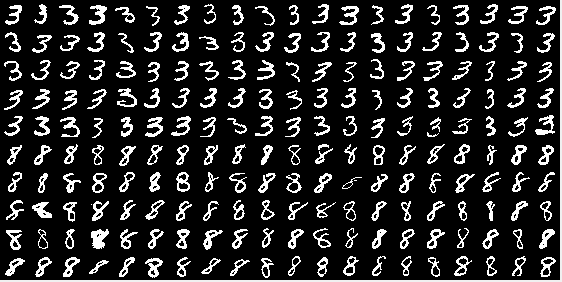
\includegraphics[width=0.85\linewidth]{training-examples.png}
\end{figure}

The function \cmd{avgImg = montageDigits(x)} additionally returns the average of all images in x. You can visualize it using \cmd{imagesc(avgImg); colormap gray}. This is useful for debugging your feature selection algorithms in decision trees. Below are the outputs of: 
\begin{itemize}
\item \cmd{avgImg = montageDigits(data.train.x)}, i.e., all training images
\item \cmd{avgImg = montageDigits(data.train.x(:,:,:, data.train.y==3)}, i.e., only the 3s
\item \cmd{avgImg = montageDigits(data.train.x(:,:,:, data.train.y==8)}, i.e., only the 8s
\end{itemize}

\begin{figure}[h]
\centering
\begin{tabular}{ccc}

\includegraphics[width=0.2\linewidth]{avgall.png} &

\includegraphics[width=0.2\linewidth]{avg3.png} &

\includegraphics[width=0.2\linewidth]{avg8.png} \\
all & 3s & 8s
\end{tabular}
\end{figure}

\newpage
\section{Decision trees}

Answer the following about decision trees.
\begin{enumerate}
\item \cmd{(4 points)} What is the accuracy of an empty decision tree on the training set? Accuracy is the fraction of the examples correctly classified. What about its accuracy on the test set? Briefly explain your answer.

\item Suppose you are allowed to ask the value of one pixel for predicting the label of the image. Which pixel should it be? This is a decision tree of depth 1.

\begin{enumerate}
\item \cmd{(15 points)} To answer this question write a function \cmd{score = scoreFeatures(x, y)}. 
The \cmd{score} is a matrix of size $28\times 28$ that corresponds to the number of examples \cmd{x} that can be correctly classified if the value of that pixel was known. 
From this find the pixel that has the highest score. 
Include the code, the score visualized as an image using \cmd{imagesc(score); colormap gray; axis image}. 
Also write down the (x,y) coordinates of pixel with the highest score and the value of the score.

\item \cmd{(5 points)} Write down the decision tree that obtains the best classification in the form of an if-then-else statement. For example, "if pixel(5,10) == 1 then predict 3, else predict 8". The exact syntax is not important.

\item \cmd{(5 points)} Apply this rule on the test set. What accuracy does this rule obtain?
\end{enumerate}

\item Compute a decision tree of depth 2 to classify the data. 
Suppose (x,y) was the pixel selected in the previous step. 
This divides the training data into two subsets, one for which pixel(x,y) = 1, and another for which pixel(x,y) = 0. 
The best pixel in the next level of the tree can be obtained by repeating the previous step for each subset of the data.
\begin{enumerate}
\item \cmd{(15 points)} Apply the above to construct the next level of the tree. Write down the resulting classifier using if-then-else statements. For example, 
\begin{verbatim}
if pixel(5,10) == 1
    if pixel(14,22) == 1
        predict 3;
    else
        predict 8;
    end
else 
    if pixel(11,6) == 1
        predict 8;
    else
        predict 3;
    end
end
\end{verbatim}
\item \cmd{(5 points)} Apply this rule on the test set. What accuracy does this rule obtain?
\end{enumerate}
\end{enumerate}

\section{Linear classifier}
The codebase includes a function: $\cmd{model=linearTrain(x, y)}$ that trains a linear classifier given features $\cmd{x}$ and labels $\cmd{y}$. The features $\cmd{x}$ are $d \times N$ dimensional and labels $\cmd{y}$ are $1 \times N$ dimensional. To use the function you have to reshape the images to a matrix where each column corresponds to a training example. The returned model has two fields: $\cmd{model.w}$ is the weight vector of size $d+1$ corresponding to weights on features and a bias term and $\cmd{model.classLabels}$ corresponding to the labels. In Python model is structured as a dictionary, so you should use $\cmd{model["weights"]}$ and $\cmd{model["classLabels"]}$.

Once the model is trained you can obtain predictions using $\cmd{ypred = linearPredict(model, x)}$. This function expects the input $\cmd{x}$ in the same format as the training data.

\begin{itemize}
\item \cmd{(10 points)} What accuracy does the linear model obtain on the test set? Include the code for training and evaluating the model.
\item \cmd{(5 points)} Visualize the positive and negative parts of the weights by reshaping the first $d$ dimensions (i.e., ignoring the bias term) as an image. You compute the positive and negative components as $\cmd{wp=w.*(w > 0)}$ and $\cmd{wn=-w.*(w < 0)}$ and using $\cmd{imagesc(reshape(wp, [28 28]))}$ to display them. In Python, you can use $\cmd{plt.imshow(wp.reshape((28, 28))}$.
\end{itemize}

\section{Nearest neighbor classifier}
\cmd{(15 points)} Using Euclidean distance between pixels as the similarity between images plot the accuracy of a k nearest-neighbor classifier for $\cmd{k=1,3,5}$ on the test set. Include the code for your implementation.

\section{Bag-of-visual-words representations}
In this part you will implement this Bag-of-visual representation by the following two steps: 1) constructing a dictionary of visual words, and 2) represent each image as a histogram over the words. The second part is counted as extra credits and you need to report the accuracy with linear classifiers to obtain the full extra credits.
\begin{itemize}
\item \cmd{[15 points]}: Implement the function \cmd{C=constructDictionary(x, K, ps)}. The function takes the entire training set \cmd{x} as input and outputs a dictionary \cmd{C} of size \cmd{ps x ps x K} where \cmd{K} is the number of visual words and each word is a patch of size \cmd{ps x ps}. To construct a dictionary, randomly draw 20 patches from each images in the training data to obtain a set of sampled patches and group all the sampled patches into \cmd{K} clusters by k-means clustering. In MATLAB, you can call the function \cmd{kmeans} for clustering. For Python users, you need the \cmd{scikit-learn} package for \cmd{sklearn.cluster.KMeans}. Take a look at the first example in the documentation\footnote{\url{https://scikit-learn.org/stable/modules/generated/sklearn.cluster.KMeans.html}}. Use \cmd{K=100} and \cmd{ps=9} and visualize the dictionary by \cmd{montageDigits} as shown in the following figure:
\begin{figure}[h]
\centering
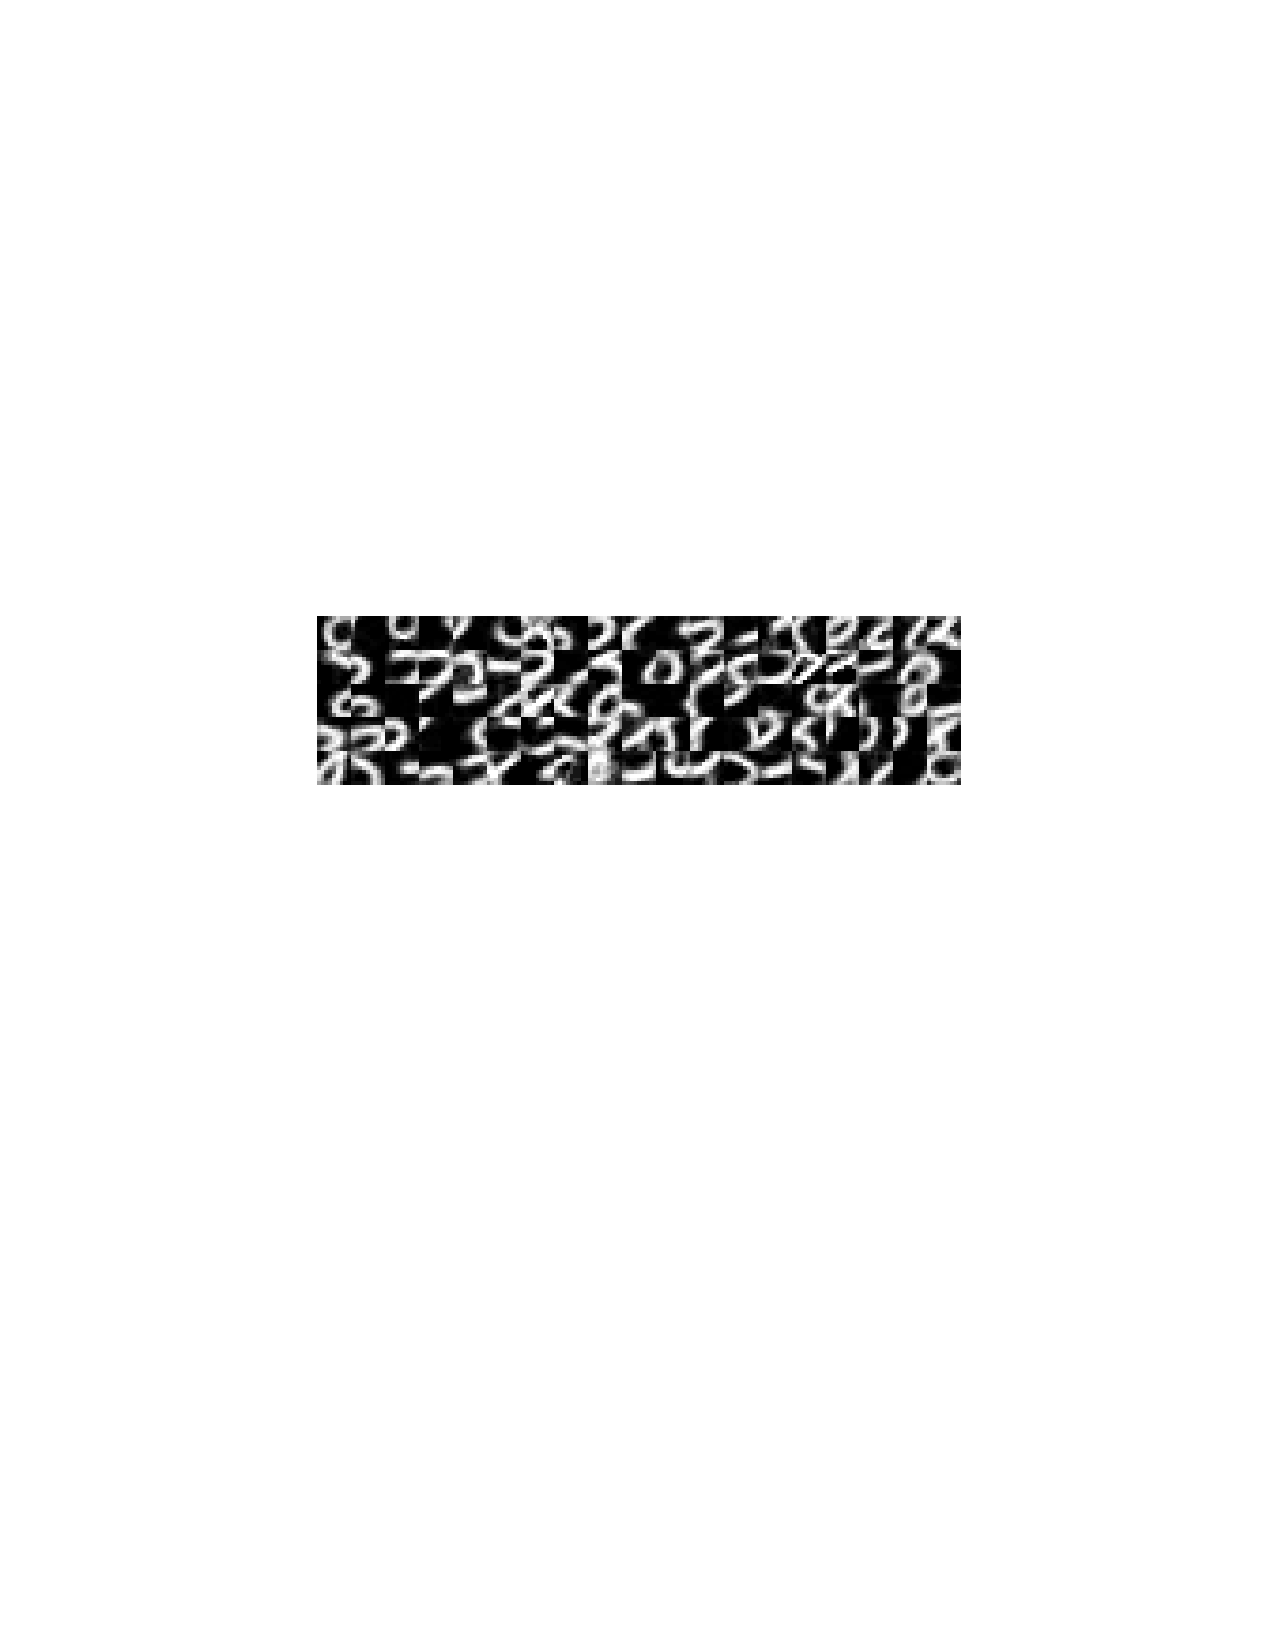
\includegraphics[trim={0cm 14cm 0cm 10cm},clip, width=\linewidth]{dictionary.pdf}
\end{figure}

Take a look at the start code \cmd{evalBoVW.m}. Include your implementation and the visualization of dictionary in your submission.

\item \textbf{Extra credits:} \cmd{[15 points]}: Implement the function \cmd{y=encodeImage(im, C)}. The function encodes the image \cmd{im} with the dictionary \cmd{C} as a histogram over the visual words. For each pixel in the image, consider the patch of size \cmd{ps x ps} centered at the pixel. The patch is assigned to the visual word with smallest sum-of-squared distance. You can ignore the pixels at the boundary if the patch is not entirely in the image. For each visual word, compute the number of patches that are assigned to it. This gives you a $K$-dimensional vector \cmd{y} where each entry is the number of patches that belong to a visual word. Encode all the images with the dictionary and train a linear classifier to classify 3 and 8. You can find more details in \cmd{evalBoVW.m}. In your submission, include your implementation and report the accuracy on test set. You should be able to get the accuracy around 97\%. 

\item \textit{Hint:}  To find the nearest visual word, you will find the function \cmd{pdist2} useful in MATLAB. The equivalent function in Python is \cmd{scipy.spatial.distance.cdist}.

\end{itemize}
\section{What to submit?}
In addition to what is required for each problem, include all the relevant code, and intermediate results needed for explaining your implementation. \textbf{Finally, congratulations on completing all the homework assignments!}

\section{Submission and rubric}

\begin{itemize}
\item Follow the outline on Gradescope for your submission. 
\item A fraction of the points for each coding assignment will be for
  readability and efficiency of your code. Thus it is important to
  properly document parts of the code you implemented.
\end{itemize}

\end{document}
